\chapter{Matrix Chain Parenthesization}

\section{Descrizione del problema}

Data una sequenza di $n$ matrici $A_1, A_2, \ldots, A_n$, vogliamo
calcolare il prodotto $A_1A_2 \ldots A_n$.\\

Possiamo calcolare quest'ultimo utilizzando come subroutine l'algoritmo
standard per moltiplicare una coppia di matrici, dopo che abbiamo posto
le opportune parentesi per eliminare qualsiasi ambiguità sul modo in cui
devono essere moltiplicate le matrici.\\ La moltiplicazione delle matrici
è associativa, quindi \textbf{tutte le parentesizzazioni forniscono lo
  stesso prodotto}.

\begin{definition}
  Un prodotto di matrici è \textbf{completamente
    parentesizzato} se è una singola matrice oppure è il prodotto, racchiuso
  tra parentesi, di due prodotti di matrici completamente parentesizzati.
\end{definition}

Per esempio, se la sequenza delle matrici è $A_1, A_2, A_3, A_4$, il
prodotto $A_1 A_2 A_3 A_4$ può essere parentesizzato in cinque modi
distinti:
\begin{itemize}
  \item $(A_1 (A_2 (A_3 A_4)))$
  \item $(A_1 ((A_2 A_3) A_4))$
  \item $((A_1 A_2 )(A_3 A_4))$
  \item $((A_1 (A_2 A_3 ))A_4)$
  \item $(((A_1 A_2) A_3 )A_4)$
\end{itemize}

Il modo in cui parentesizziamo una sequenza di matrici può avere un
impatto notevole sul costo per calcolare il prodotto.\\

L'algoritmo standard di moltiplicazioni tra matrici è dato dal seguente
pseudocodice:

\begin{lstlisting}[language=Python, mathescape=true]
function Matrix-Multiply(A, B) {
 Require: Matrices A, B with A.columns = B.rows

 Let C be a new A.rows $\times$ B.columns matrix

 for i $\leftarrow$ 1 $\ldots$ A.rows do
   for j $\leftarrow$ 1 $\ldots$ B.columns do
     Cij $\leftarrow$ 0
     for k $\leftarrow$ 1 $\ldots$ A.columns do
       Cij $\leftarrow$ Cij + Aik $\cdot$ Bkj

 return C
}
\end{lstlisting}

\subsection{Costo}

\begin{itemize}
  \item Tre cicli nidificati: $O(A.righe \cdot B.colonne \cdot A.colonne)$
  \item Numero di moltiplicazioni: \emph{A.righe $\cdot$ B.colonne $\cdot$ A.colonne}
  \item Moltiplicazione di due matrici $n \times n$: runtime $O(n^3)$
\end{itemize}

%% TODO: ricontrollare riga 8 dell'algoritmo
\paragraph*{Nota:}
\begin{itemize}
  \item Possiamo moltiplicare due matrici soltanto se sono
        \textbf{compatibili}: il numero di colonne di $A$ deve essere uguale
        al numero di righe di $B$.
  \item Se $A$ è una matrice $p \times q$ e
        $B$ è una matrice $q \times r$, la matrice risultante $C$ è una
        matrice $p \times r$.
  \item Il tempo per calcolare $C$ è dato dal numero di prodotti scalari, che
        è $p \cdot q \cdot r$ (riga 8 dell'algoritmo).
\end{itemize}

Per mostrare come il costo per moltiplicare le matrici dipenda dallo
schema di parentesizzazione, consideriamo il problema di moltiplicare
una sequenza di tre matrici $A_1, A_2, A_3$. Supponiamo che le
dimensioni siano rispettivamente \texttt{10\ x\ 100},
\texttt{100\ x\ 5}, \texttt{5\ x\ 50}. Se moltiplichiamo secondo lo
schema di parentesizzazione $((A_1 A_2 )A_3)$ eseguiamo
\texttt{10\ x\ 100\ x\ 5\ =\ 5000} prodotti scalari per calcolare la
matrice \texttt{10\ x\ 5} risultante dal prodotto $A_1 A_2$, più
altri \texttt{10\ x\ 5\ x\ 50\ =\ 2500} prodotti scalari per
moltiplicare questa matrice per $A_3$, per un totale di 7500 prodotti
scalari. Se invece moltiplichiamo secondo lo schema di parentesizzazione
$(A_1 (A_2 A_3))$ eseguiamo \texttt{100\ x\ 5\ x\ 50\ =\ 25000}
prodotti scalari per calcolare la matrice \texttt{100\ x\ 50} risultante
dal prodotto $A_2 A_3$, più altri
\texttt{10\ x\ 100\ x\ 50\ =\ 50000} prodotti scalari per moltiplicare
questa matrice per $A_1$, per un totale di 75000 prodotti scalari.\\
Quindi il calcolo della moltiplicazione delle matrici è 10 volte più
rapido con il primo schema di parentesizzazioni.

Il \textbf{problema della parentesizzazione tra matrici} può essere
descritto in questo modo:
\begin{myblockquote}
  Data una sequenza di $n$
  matrici $A_1, A_2, \ldots, A_n$, dove la matrice $A_i$ ha dimensioni
  $p_{i-1} \times p_i$ per $i = 1,2, \ldots,n$, determinare lo schema di
  parentesizzazione completa del prodotto $A_1A_2 \ldots A_n$ che minimizza
  il numero di prodotti scalari.
\end{myblockquote}


\subsection{Goal}

È importante notare che, nel problema della moltiplicazione di una
sequenza di matrici, \textbf{non vengono effettivamente moltiplicate le
  matrici}. Il nostro \textbf{obiettivo è soltanto quello di determinare
  un ordine di moltiplicazione delle matrici che ha il costo minimo}.\\
Tipicamente, il tempo impiegato per determinare quest'ordine ottimo è
più che ripagato dal tempo risparmiato successivamente per eseguire
effettivamente i prodotti delle matrici (per esempio, eseguire soltanto
7500 prodotti, anziché 75000).\\
\\
Vogliamo tuttavia dimostrare che un controllo esaustivo di tutti i
possibili schemi di parentesizzazione non ci consente di ottenere un
algoritmo efficiente. Indichiamo con $P(n)$ il numero di
parentesizzazioni alternative di una sequenza di $n$ matrici.
\begin{itemize}
  \item Quando
        $n=1$, c'è una sola matrice e, quindi un solo schema di
        parentesizzazione.
  \item Quando $n \ge 2$, un prodotto di matrici
        completamente parentesizzato è il prodotto di due sottoprodotti di
        matrici completamente parentesizzati e la suddivisione fra i due
        sottoprodotti può avvenire fra la $k$-esima e la $(k+1)$-esima matrice per
        qualsiasi $k=1,2,\ldots,n-1$.
\end{itemize}

Quindi otteniamo la seguente ricorrenza:

%% TODO: riscrivere in LaTex
\begin{figure}[H]
  \centering
  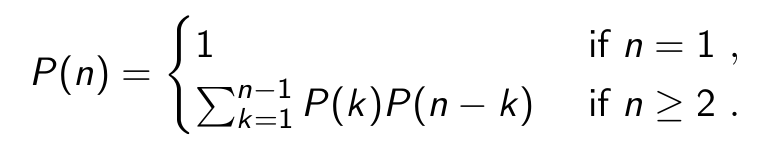
\includegraphics[width=10cm, keepaspectratio]{capitoli/programmazione_dinamica/imgs/matrix1.png}
  \caption{Sequenza: 1, 1, 2, 5, 14, 42, 132, 429, 1430, 4862, 16796, 58786, 208012, 742900,
    $\ldots$}
\end{figure}

Si può dimostrare che ci sono $\Omega(2^n)$ combinazioni.
Un algoritmo efficiente quindi non può provare tutte le possibili
combinazioni.

\section{Applicare la programmazione dinamica}

Seguiremo un procedimento di quattro fasi (classico della programmazione
dinamica):
\begin{enumerate}
  \item Caratterizzare la struttura di una soluzione ottima
  \item Definire in modo ricorsivo il valore di una soluzione ottima
  \item Calcolare il valore di una soluzione ottima
  \item Costruire una soluzione ottima dalle informazioni calcolate
\end{enumerate}

\subsection{Struttura di una parentesizzazione ottima}

Per comodità adottiamo la notazione $A_{i..j}$ dove $i \le j$, per
la matrice che si ottiene calcolando il prodotto
$A_i A_{i+1} \ldots A_j$. Notate che, se il problema non è banale, cioè
$i < j$, allora qualsiasi parentesizzazione del prodotto
$A_i A_{i+1} \ldots A_j$ deve suddividere il prodotto fra $A_k$ e
$A_{k+1}$ per qualche intero $k$ nell'intervallo $i \le k < j$,
ovvero:
\begin{itemize}
  \item per qualche valore di $k$, prima calcoliamo le matrici
        $A_{i..k}$ e $A_{k+1..j}$
  \item e, poi, le moltiplichiamo per ottenere
        il prodotto finale $A_{i..j}$
\end{itemize}

Il costo di questa parentesizzazione è, quindi, il costo per calcolare
la matrice $A_{i..k}$, più il costo per calcolare la matrice
$A_{k+1..j}$, più il costo per per moltiplicare queste due matrici.


\subsubsection{Defininizione della sottostruttura}

\begin{myblockquote}
  Supponiamo che una parentesizzazione ottima $A_i A_{i+1} \ldots A_j$
  suddivida \linebreak il prodotto fra $A_k$ e $A_{k+1}$. Allora la
  parentesizzazione della prima sottosequenza $A_i A_{i+1} \ldots A_k$
  all'interno di questa parentesizzazione ottima di
  $A_i A_{i+1} \ldots A_j$, deve essere una parentesizzazione ottima di
  $A_i A_{i+1} \ldots A_k$.
\end{myblockquote}

\textbf{Possiamo quindi costruire una soluzione ottima di un'istanza del
  problema della moltiplicazione di una sequenza di matrici suddividendo
  il problema in due sottoproblemi} (quelli della parentesizzazione ottima
$A_i A_{i+1} \ldots A_k$ e $A_{k+1} A_{k+2} \ldots A_j$ ), trovando le
soluzioni ottime delle istanze dei sottoproblemi e, infine,
\textbf{combinando} \textbf{le soluzioni ottime dei sottoproblemi}.

\subsection{Soluzione in modo ricorsivo}

Scegliamo come sottoproblemi i problemi per determinare il costo minimo
di una parentesizzazione $A_i A_{i+1} \ldots A_j$ per
$1 \le i \le j \le n$.\\ Sia \texttt{m[i,j]} \textbf{il numero
  minimo di prodotti scalari richiesti per calcolare la matrice}
$A_{i..j}$; per il problema principale, il costo del metodo più
economico per calcolare $A_{1..n}$ sarà quindi \texttt{m[1,n]}.
Possiamo definire \texttt{m[i,j]} ricorsivamente in questo modo:
\begin{itemize}
  \item Se $i = j$, il problema è banale; la sequenza è formata da una matrice
        $A_{i..i} = A_i$, quindi non occorre eseguire alcun prodotto scalare.
        Allora \texttt{m[i,i]} = 0 per $i=1,2,\ldots,n$.
  \item Per calcolare \texttt{m[i,j]} quando $i < j$, sfruttiamo la struttura di una
        soluzione ottima ottenuta nella fase 1.
        Supponiamo che la parentesizzazione ottima suddivida il prodotto
        $A_i A_{i+1} \ldots A_j$ fra $A_k$ e $A_{k+1}$, dove $i \le k < j$.
        Quindi \texttt{m[i,j]} è uguale al costo minimo per calcolare i
        sottoprodotti $A_{i..k}$ e $A_{k+1..j}$, più il costo per
        moltiplicare queste due matrici. Ricordando che ogni matrice $A_i$ è
        $p_{i-1} \times p_i$, il calcolo del prodotto delle matrici
        $A_{i..k} A_{k+1..j}$ richiede $p_{i-1} p_k p_j$ prodotti scalari.
        Quindi otteniamo: $m[i,j] = m[i,k] + m[k+1,j] + p_{i-1} p_k p_j$
\end{itemize}

Questa equazione ricorsiva suppone che sia noto il valore di $k$, che
invece non conosciamo. Notiamo tuttavia, che ci sono soltanto $j-i$
valori possibili per $k$, ovvero $k=i, i+1, \ldots, j-1$. Poiché la
parentesizzazione ottima deve utilizzare uno di questi valori di $k$,
dobbiamo semplicemente controllarli tutti per trovare il migliore.
Quindi, la nostra definizione ricorsiva per il costo minimo di una
parentesizzazione del prodotto $A_i A_{i+1} \ldots A_j$ diventa:

%% TODO: riscrivere in LaTex
\begin{figure}[H]
  \centering
  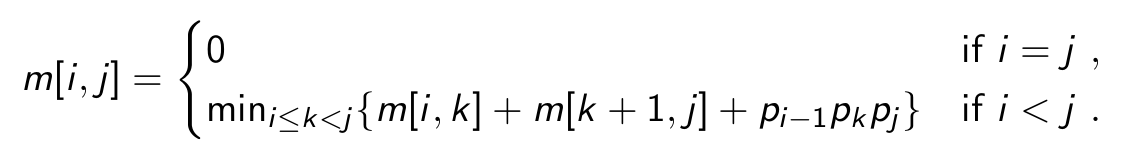
\includegraphics[width=15cm, keepaspectratio]{capitoli/programmazione_dinamica/imgs/matrix2.png}
\end{figure}

I valori \texttt{m[i,\ j]} sono i costi delle soluzioni ottime dei
sottoproblemi, ma essi non ci forniscono tutte le informazioni
necessarie a ricostruire la soluzione ottima. Per poterlo fare definiamo
\texttt{s[i,j]} come il valore $k$ in cui è stato suddiviso il
prodotto $A_{i} A_{i+1} \ldots A_j$ per ottenere una parentesizzazione
ottima. Ovvero, \texttt{s[i,j]} è uguale a un valore $k$ tale che
$m[i,j] = m[i,k] + m[k+1,j] + p_{i-1} p_k p_j$

\subsection{Calcolo dei costi ottimi}

Osserviamo che ci sono relativamente pochi problemi distinti: un
problema per ogni possibile scelta di $i$ e $j$, con
$1 \le i \le j \le n$ per un totale di $O(n^2)$. Un algoritmo
ricorsivo può incontrare ciascun sottoproblema più volte nelle varie
diramazioni del suo albero di ricorsione. \textbf{Questa proprietà dei
  sottoproblemi che si ripresentano è la seconda caratteristica peculiare
  dell'applicabilità della programmazione dinamica} (la prima è la
sottostruttura ottima).\\

Anziché calcolare la soluzione della ricorrenza ricorsivamente,
calcoliamo il costo ottimale applicando un metodo tabulare Bottom-Up.\\
Implementiamo quest'ultimo con la procedura \texttt{Matrix-Chain-Order}
riportata qui di seguito. Questa procedura assume che la matrice $A_i$
abbia dimensione $p_{i-1} \times p_i$ per $i=1,2,\ldots,n$. L'input è una
sequenza $p = p_0, p_1, \ldots, p_n$, dove \texttt{p.length} $= n+1$.\\
La procedura usa una tabella ausiliaria \texttt{m[1..n,\ 1..n]} per
memorizzare i costi \texttt{m[i,j]} e una tabella ausiliaria
\texttt{s[1..n,\ 1..n]} che registra l'indice $k$ cui corrisponde
il costo ottimo nel calcolo \texttt{m[i,j]}. La tabella \texttt{s}
sarà poi utilizzata per costruire una soluzione ottima.\\

Per implementare correttamente il metodo Bottom-Up dobbiamo determinare
quali posizioni nella tabella sono utilizzate nel calcolo di
\texttt{m[i,j]}.\\ L'equazione ricorsiva, definita precedentemente,
indica che il costo \texttt{m[i,j]} per calcolare il prodotto di
$j-i+1$ matrici dipende soltanto dai costi per calcolare prodotti di
sequenze di meno di $j-i+1$ matrici. Ovvero, per $k=i,i+1,\ldots,j-1$,
la matrice $A_{i..k}$ è un prodotto di $k-i+1 < j-i+1$ matrici e la
matrice $A_{k+1..j}$ è un prodotto di $j-k < j-i+1$ matrici.\\

L'algoritmo dovrebbe riempire la tabella \texttt{m} in modo da risolvere
il problema della parentesizzazione di sequenze di matrici di lunghezza
crescente. Per il sottoproblema della parentesizzazione ottima della
sequenza di matrici $A_i A_{i+1} \ldots A_j$, assumiamo come dimensione
del problema la lunghezza $j-i+1$ della sequenza.


\section{Bottom-Up Approach}

\begin{lstlisting}[language=Python, mathescape=true]
function Matrix-Chain-Order(p) {
  matrix Ai has dimensions p(i-1) $\times$ p(i)
  n = p.length - 1

  Let m[1$\ldots$n,1$\ldots$n] and s[1$\ldots$n,1$\ldots$n] be new arrays

  for i $\leftarrow$ 1 $\ldots$ n do
	  m[i,i] $\leftarrow$ 0
  for l $\leftarrow$ 2$\ldots$n do                # l = chain length
	  for i $\leftarrow$ 1 $\ldots$ n - l + 1 do    # left position 
		  j $\leftarrow$ i + l - 1              # right position
		  m[i,j] $\leftarrow$ $\infty$
		  for k $\leftarrow$ i $\ldots$ j - 1 do
            q  = m[i,k] + m[k +1,j] + pi-1 pk pj
            if q $<$ m[i,j]
              m[i,j] = q
              s[i,j] = k

  return m and s
}
\end{lstlisting}

L'algoritmo prima calcola \texttt{m[i,i]} $= 0$ per
$i=1, 2,\ldots,n$ (i costi minimi per sequenze di lunghezza $l=1$). Poi
usa la ricorrenza per calcolare \texttt{m{[}i,i+1{]}} per
$i=1,2,\ldots,n-1$ (i costi minimi per sequenze di lunghezza $l=2$)
durante la prima esecuzione del ciclo \texttt{for}. Nella seconda
iterazione del ciclo, l'algoritmo calcola \texttt{m{[}i,\ i+2{]}} per
$i =1,2,\ldots,n-2$ (i costi minimi per cammini di lunghezza $l=3$) e
così via. In ciascun passo, il costo calcolato \texttt{m{[}i,j{]}}
dipende soltanto dagli elementi della tabella \texttt{m{[}i,k{]}} e
\texttt{m{[}k+1,j{]}} già calcolati.


\subsection{Costo}

Da un semplice esame dalla struttura annidata dei cicli della
procedura \texttt{Matrix-Chain-Order} si deduce che il \textbf{tempo
  di esecuzione dell'algoritmo è pari a} $O(n^3)$. I cicli hanno tre
livelli di annidamento e ogni indice di ciclo ($l,i \text{ e } k$)
assume al massimo $n-1$ valori.\\
L'algoritmo richiede \textbf{in spazio} $O(n^2)$ per memorizzare le
tabelle \texttt{m} e \texttt{s}.\\

Quindi, la procedura \texttt{Matrix-Chain-Order} \textbf{è molto più
  efficiente del metodo con tempo esponenziale che elenca tutte le
  possibili parentesizzazioni controllandole una per una}.


\section{Costruire una soluzione ottima}

La procedura \texttt{Matrix-Chain-Order}, determina il numero ottimo di prodotti
scalari richiesti per moltiplicare una sequenza di matrici, ma non mostra
direttamente come moltiplicare le matrici. La tabella
\texttt{s{[}1,..n,1,..n{]}} ci fornisce le informazioni per farlo. Ogni
posizione \texttt{s{[}i,j{]}} registra quel valore di $k$ per il quale la
parentesizzazione ottima di $A_i A_{i+1}\ldots A_j$ suddivide il prodotto fra
$A_k$ e $A_{k+1}$.\\

Quindi, sappiamo che il prodotto finale delle matrici nel calcolo di
$A_{1..n}$ è \linebreak $A_{1..s[1,n]} A_{s[1,n]+1..n}$. I prodotti precedenti
possono essere calcolati ricorsivamente perché
\texttt{s{[}i,\ s{[}i,n{]}{]}} determina l'ultimo prodotto nel calcolo
di $A_{s[1,n]+1..n}$. La seguente procedura ricorsiva produce una
parentesizzazione ottima di ($A_i$, $A_{i+1}$,\ldots,$A_j$) dati
gli indici $i$ e $j$ e la tabella \texttt{s} (calcolata da
\texttt{Matrix-Chain-Order}). La chiamata iniziale di
\texttt{Print-Optimal-Parens(s,\ 1,\ n)} produce una parentesizzazione
ottima di ($A_1$, $A_2$,\ldots,$A_n$).\\

\begin{lstlisting}[language=Python, mathescape=true]
function Print-Optimal-Parens(s, 1, n) {
  Require: Array s, positions i, j

  if i = j then
    print "Ai "

  else
    print "("
    Print-Optimal-Parens(s, i, s[i, j])
    Print-Optimal-Parens(s, s[i, j] + 1, j)
    print ")"
}
\end{lstlisting}
\newpage
\section{Riepilogo}

\begin{itemize}
  \item
        L'obiettivo è minimizzare i prodotti scalari con parentesizzazione
  \item
        $m[i,j] = \min_{i \leq k < j} (m[i,k] + m[k+1, j] + p_{i-1} p_k p_j)$
  \item
        spazio necessario: ho bisogno di una matrice (triangolare superiore)
        per ricordarmi i valori calcolati precedentemente, riempita per
        diagonali.
  \item
        spazio matrice $n \times n$ : \textbf{SPAZIO =} $O(n^2)$
  \item
        per ogni cella pago $n$: \textbf{TEMPO =} $O(n^3)$
  \item
        per ricostruire la soluzione: \textbf{SPAZIO} = $O(n^2)$ uso una
        matrice dove segno quale $k$ per ogni $(i,j)$ ha dato il risultato
        migliore
\end{itemize}
